\documentclass{article}
\usepackage{amsmath, amssymb, tikz}
\usetikzlibrary{automata, positioning, arrows}
\usepackage{hyperref}

\title{\textbf{Report: Programming with Automata}}
\author{Max Randall}
\date{\today}

\begin{document}

\maketitle

\tableofcontents

\section{Introduction}
In this homework, we explore the implementation of deterministic finite automata (DFAs) in Python. 
We will go beyond the simple graphical representation of DFAs and build them using Python types.

\newpage

\section{Programming with Automata}
We will impliment the follwing DFAs in Python using this DFA class:

\begin{verbatim}
class DFA:

    def __init__(self, Q, Sigma, delta, q0, F):
        self.Q = Q  # Set of states
        self.Sigma = Sigma  # Alphabet
        self.delta = delta  # Transition function (dict)
        self.q0 = q0  # Initial state
        self.F = F  # Set of accepting states

    def __repr__(self):
        return f"DFA({self.Q},\n\t{self.Sigma},\n\t{self.delta},
                      \n\t{self.q0},\n\t{self.F})"

    def run(self, w):
        current_state = self.q0  # Start at initial state
        loop = 0
        for symbol in w:
            loop += 1
            if symbol not in self.Sigma:
                return False  # Reject if symbol is not in the alphabet
            if (current_state, symbol) not in self.delta:
                return False  # Reject if there's no valid transition
            current_state = self.delta[(current_state, symbol)]  # Move to next state
        
        return current_state in self.F  # Accept if final state is in F
\end{verbatim}

\newpage

\subsection*{Exercise 1: Word Processing with DFAs}
\textbf{Given DFAs $\mathcal{A}_1$ and $\mathcal{A}_2$:}

\begin{center}
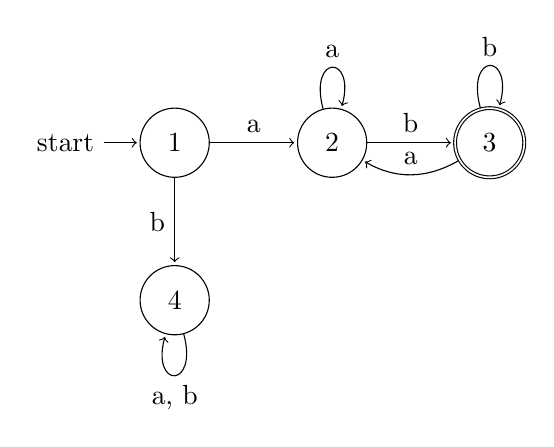
\begin{tikzpicture}[shorten >=1pt, node distance=2cm, on grid, auto] 
   \node[state, initial] (q_1) {1}; 
   \node[state] (q_2) [right=of q_1] {2}; 
   \node[state, accepting] (q_3) [right=of q_2] {3}; 
   \node[state] (q_4) [below=of q_1] {4};

   \path[->] 
    (q_1) edge [above] node {a} (q_2)
          edge [left] node {b} (q_4)
    (q_2) edge [loop above] node {a} ()
          edge [above] node {b} (q_3)
    (q_3) edge [bend left, above] node {a} (q_2)
          edge [loop above] node {b} ()
    (q_4) edge [loop below] node {a, b} (); 
\end{tikzpicture}

\textit{Automaton $\mathcal{A}_1$}
\end{center}

\begin{center}
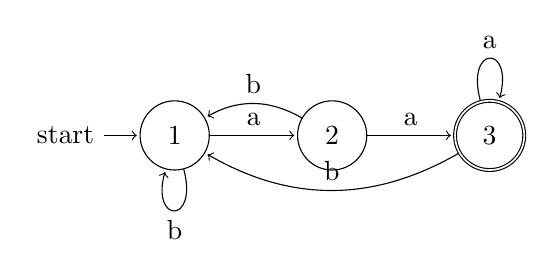
\begin{tikzpicture}[shorten >=1pt, node distance=2cm, on grid, auto] 
   \node[state, initial] (q_1) {1}; 
   \node[state] (q_2) [right=of q_1] {2}; 
   \node[state, accepting] (q_3) [right=of q_2] {3}; 

   \path[->] 
    (q_1) edge [above] node {a} (q_2)
          edge [loop below] node {b} ()
    (q_2) edge [above] node {a} (q_3)
          edge [bend right, above] node {b} (q_1)
    (q_3) edge [loop above] node {a} ()
          edge [bend left, above] node {b} (q_1);
\end{tikzpicture}

\textit{Automaton $\mathcal{A}_2$}
\end{center}

Here is how we initialize the DFAs in python:

\begin{verbatim}
    # DFA A1
    Q = {1,2,3,4}
    Sigma = {'a','b'}
    delta = {(1,'a'):2, (1,'b'):4, (2,'a'):2, (2,'b'):3, 
             (3,'a'):2, (3,'b'):2, (4,'a'):4, (4,'b'):4}
    q0 = 1
    F = {3}
    A1 = dfa.DFA(Q, Sigma, delta, q0, F)
    
    # DFA A2
    Q = {1,2,3}
    Sigma = {'a','b'}
    delta = {(1,'a'):2, (1,'b'):1, (2,'a'):3, (2,'b'):1,
             (3,'a'):3, (3,'b'):1}
    q0 = 1
    F = {3}
    A2 = dfa.DFA(Q, Sigma, delta, q0, F)
\end{verbatim}

\newpage

\section{Exercise 4: Complement DFA}
Construct an automaton $A_0$ such that $A_0$ accepts exactly the words that $A$ refuses and vice versa. Implement the method \texttt{refuse} in \texttt{dfa.py} to return this new DFA.

\begin{center}
    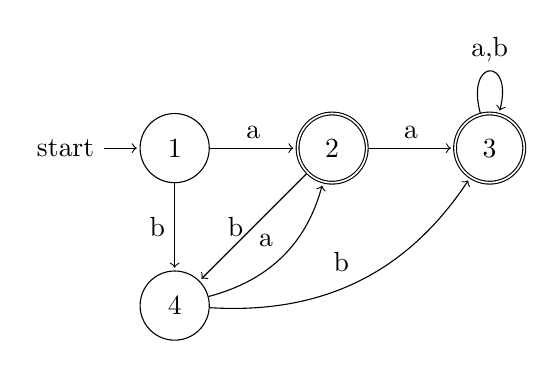
\begin{tikzpicture}[shorten >=1pt, node distance=2cm, on grid, auto] 
    \node[state, initial] (q_1) {1}; 
    \node[state, accepting] (q_2) [right=of q_1] {2}; 
    \node[state, accepting] (q_3) [right=of q_2] {3}; 
    \node[state] (q_4) [below=of q_1] {4};

    \path[->] 
        (q_1) edge [above] node {a} (q_2)
            edge [left] node {b} (q_4)
        (q_2) edge [above] node {a} (q_3)
            edge [left] node {b} (q_4)
        (q_3) edge [loop above] node {a,b} ()
        (q_4) edge [bend right] node {a} (q_2)
            edge [bend right] node {b} (q_3);
    \end{tikzpicture}
\end{center}

To construct an automaton $A_0$ that only accepts words that $A$ refuses we can simply
swap the accepting states with the previously not accepted states.

\begin{center}
    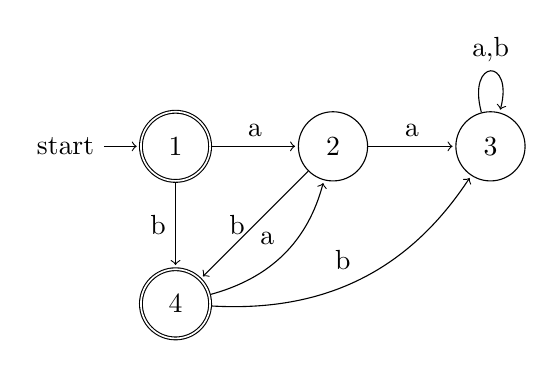
\begin{tikzpicture}[shorten >=1pt, node distance=2cm, on grid, auto] 
       \node[state, initial, accepting] (q_1) {1}; 
       \node[state] (q_2) [right=of q_1] {2}; 
       \node[state] (q_3) [right=of q_2] {3}; 
       \node[state, accepting] (q_4) [below=of q_1] {4};
    
       \path[->] 
            (q_1) edge [above] node {a} (q_2)
                edge [left] node {b} (q_4)
            (q_2) edge [above] node {a} (q_3)
                edge [left] node {b} (q_4)
            (q_3) edge [loop above] node {a,b} ()
            (q_4) edge [bend right] node {a} (q_2)
                edge [bend right] node {b} (q_3);
    \end{tikzpicture}
\end{center}

We can represent this operation with a refuse() function in Python.
\begin{verbatim}
def refuse(A):
    """Constructs a DFA A0 that accepts exactly the words that A refuses and vice versa."""
    Q0 = A.Q
    Sigma0 = A.Sigma
    delta0 = A.delta
    q0_0 = A.q0
    F0 = Q0 - A.F  # Complement of the accepting states

    return dfa.DFA(Q0, Sigma0, delta0, q0_0, F0)
\end{verbatim}

\newpage

\section*{Summary of chapter 2.2.4}

A \textbf{Deterministic Finite Automaton (DFA)} is a formal model of computation that processes input sequences while maintaining a single, well-defined state at any given time. The term "deterministic" means that for each input symbol, the automaton transitions to exactly one state.

\subsection*{Components of a DFA}
A DFA consists of five elements:
\begin{enumerate}
    \item \textbf{Finite set of states} \( Q \)
    \item \textbf{Finite set of input symbols} \( \Sigma \)
    \item \textbf{Transition function} \( \delta \): \( Q \times \Sigma \to Q \), mapping states and inputs to new states
    \item \textbf{Start state} \( q_0 \in Q \)
    \item \textbf{Set of accepting states} \( F \subseteq Q \)
\end{enumerate}

A DFA is often represented as a \textbf{five-tuple}:
\[
A = (Q, \Sigma, \delta, q_0, F)
\]

\subsection*{Processing Strings}
The DFA starts in \( q_0 \) and processes an input string sequentially. The transition function determines the next state. If, after processing the entire string, the DFA reaches a state in \( F \), the string is \textbf{accepted}; otherwise, it is \textbf{rejected}.

\subsection*{Representations}
DFAs can be represented in multiple ways:
\begin{itemize}
    \item \textbf{Transition diagrams:} Directed graphs with labeled edges.
    \item \textbf{Transition tables:} Tabular representation of \( \delta \).
\end{itemize}

DFAs define \textbf{formal languages} by recognizing sets of accepted strings.

\newpage

\subsection{Exercise 2.4.4}

\textbf{(a) DFA for strings ending in 00}
\begin{center}
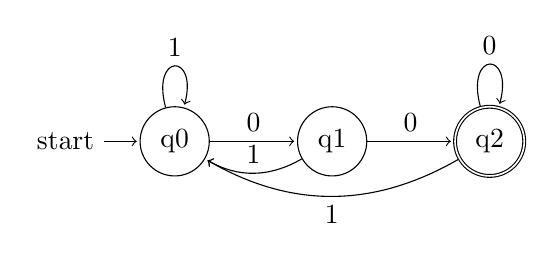
\begin{tikzpicture}[shorten >=1pt, node distance=2cm, on grid, auto]
    \node[state, initial] (q0) {q0};
    \node[state] (q1) [right=of q0] {q1};
    \node[state, accepting] (q2) [right=of q1] {q2};

    \path[->] 
        (q0) edge [loop above] node {1} ()
             edge [above] node {0} (q1)
        (q1) edge [above] node {0} (q2)
             edge [bend left, above] node {1} (q0)
        (q2) edge [loop above] node {0} ()
             edge [bend left] node {1} (q0);
\end{tikzpicture}
\end{center}

\textbf{(b) DFA for strings containing 000 as a substring}
\begin{center}
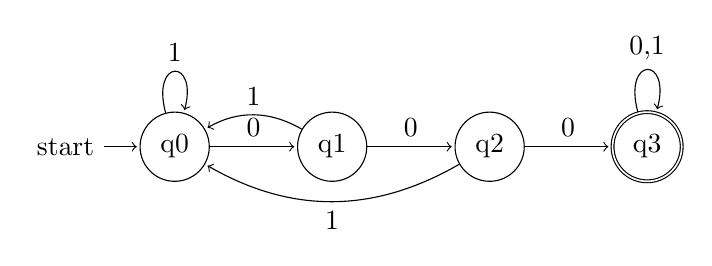
\begin{tikzpicture}[shorten >=1pt, node distance=2cm, on grid, auto]
    \node[state, initial] (q0) {q0};
    \node[state] (q1) [right=of q0] {q1};
    \node[state] (q2) [right=of q1] {q2};
    \node[state, accepting] (q3) [right=of q2] {q3};

    \path[->]
        (q0) edge [loop above] node {1} ()
             edge [above] node {0} (q1)
        (q1) edge [above] node {0} (q2)
             edge [bend right, above] node {1} (q0)
        (q2) edge [above] node {0} (q3)
             edge [bend left, below] node {1} (q0)
        (q3) edge [loop above] node {0,1} (); 
\end{tikzpicture}
\end{center}

\textbf{(c) DFA for strings containing 011 as a substring}
\begin{center}
    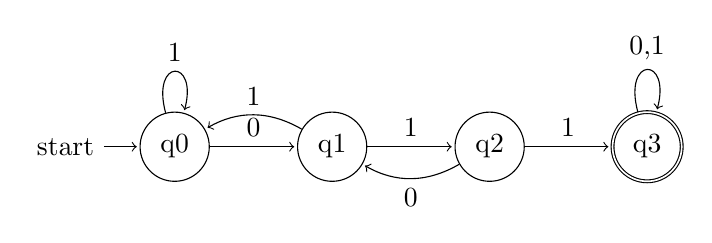
\begin{tikzpicture}[shorten >=1pt, node distance=2cm, on grid, auto]
        \node[state, initial] (q0) {q0};
        \node[state] (q1) [right=of q0] {q1};
        \node[state] (q2) [right=of q1] {q2};
        \node[state, accepting] (q3) [right=of q2] {q3};
    
        \path[->]
            (q0) edge [loop above] node {1} ()
                 edge [above] node {0} (q1)
            (q1) edge [above] node {1} (q2)
                 edge [bend right, above] node {1} (q0)
            (q2) edge [above] node {1} (q3)
                 edge [bend left, below] node {0} (q1)
            (q3) edge [loop above] node {0,1} (); 
    \end{tikzpicture}
    \end{center}

\newpage

\section{Conclusion}
\maketitle

A \textbf{Deterministic Finite Automaton (DFA)} is a theoretical computational model used to recognize formal languages. A DFA consists of a finite set of states \( Q \), an input alphabet \( \Sigma \), a transition function \( \delta: Q \times \Sigma \to Q \), a start state \( q_0 \), and a set of accepting states \( F \). The machine processes strings sequentially, transitioning between states according to \( \delta \). If, after consuming the entire string, the DFA ends in an accepting state, the input is accepted; otherwise, it is rejected. DFAs can be represented using transition diagrams or transition tables, which illustrate how states change based on input symbols. The concept of an extended transition function allows DFAs to process entire strings iteratively. Examples of DFAs include those recognizing substrings like "01" or enforcing conditions such as even parity of 0s and 1s.

The Python implementation models a DFA using a \texttt{DFA} class, which defines the state set, alphabet, transitions, initial state, and accepting states. The \texttt{run} method processes input strings and determines acceptance based on the transition function. Additionally, the \texttt{refuse} function constructs the complement DFA by inverting the accepting and refusing states, accepting only the words that the original DFA rejects. Several DFAs are defined and tested against a set of generated words, demonstrating their functionality. This implementation provides a practical means of experimenting with DFAs, allowing for the exploration of language recognition, state transitions, and DFA complement operations in a programmatic way.

\textbf{An Interesting Question: } How can the DFA implementation be optimized to handle extremely long input strings efficiently, considering that DFA state transitions form a directed graph with \( O(V + E) \) complexity?
\newpage

\begin{thebibliography}{9}
\bibitem{hopcroft} Hopcroft, J. E., Motwani, R., Ullman, J. D. \textit{Introduction to Automata Theory, Languages, and Computation}. Pearson, 2007.
\end{thebibliography}

\end{document}
